\documentclass[sigconf]{acmart}

%%
%% \BibTeX command to typeset BibTeX logo in the docs
\AtBeginDocument{%
  \providecommand\BibTeX{{%
    Bib\TeX}}}

% no “Permission to make digital or hard copies…” footnote:
\renewcommand\footnotetextcopyrightpermission[1]{}

% 2) Kill the “ACM Reference Format” block:
\settopmatter{printacmref=false}

% 3) Kill the default conference banner:
%    acmConference is defined as \newcommand\acmConference[4][]{…}
%    so when you redefine it you must keep the optional argument slot:
\renewcommand\acmConference[4][]{}%

% 4) Kill the Received/revised/accepted line:
%    (either remove your \received{…} call entirely, or blank it here)
\renewcommand\received[2][]{}%

% enable printing of page‑numbers
\settopmatter{printfolios=true}

% load fancyhdr (acmart already loads it, but we still need to configure it)
\usepackage{fancyhdr}

% clear out existing header/footer settings
\fancyhf{} 

% put the page number on the right of the footer
\fancyfoot[R]{\thepage}

% switch to the fancy style
\pagestyle{fancy}

% no header rule (and no header content)
\renewcommand{\headrulewidth}{0pt}
\renewcommand{\footrulewidth}{0pt}

% switch to this style for all pages
\pagestyle{fancy}

\makeatletter
% Redefine ACM's standardpagestyle to be “completely empty header” + “page number at bottom right”
\fancypagestyle{standardpagestyle}{%
  \fancyhf{}% clear all header/footer fields
  \fancyfoot[R]{\thepage}% page number on right of footer
  \renewcommand{\headrulewidth}{0pt}% no header rule
  \renewcommand{\footrulewidth}{0pt}% no footer rule
}
% Make that the active page style from the very first page on
\AtBeginDocument{%
  \pagestyle{standardpagestyle}%
}
\makeatother


%% end of the preamble, start of the body of the document source.
\begin{document}

%%
%% The "title" command has an optional parameter,
%% allowing the author to define a "short title" to be used in page headers.
\title{Full-Field Trajectory Prediction in the NFL Using LSTM and Transformer Models}

%%
%% The "author" command and its associated commands are used to define
%% the authors and their affiliations.
%% Of note is the shared affiliation of the first two authors, and the
%% "authornote" and "authornotemark" commands
%% used to denote shared contribution to the research.
\author{46679}
\affiliation{%
  \institution{London School of Economics and Political Science}
  \city{London}
  \country{UK}
}

\author{38682}
\affiliation{%
  \institution{London School of Economics and Political Science}
  \city{London}
  \country{UK}
}

\author{37269}
\affiliation{%
  \institution{London School of Economics and Political Science}
  \city{London}
  \country{UK}
}

\author{40658}
\affiliation{%
 \institution{London School of Economics and Political Science}
 \city{London}
 \country{UK}}

%%
%% By default, the full list of authors will be used in the page
%% headers. Often, this list is too long, and will overlap
%% other information printed in the page headers. This command allows
%% the author to define a more concise list
%% of authors' names for this purpose.
\renewcommand{\shortauthors}{LSE}

%%
%% The abstract is a short summary of the work to be presented in the
%% article.
\begin{abstract}
American football's unique start-stop rhythm, combined with the complexity of "pre-snap motion," creates a rich strategic layer that distinguishes it from more continuously flowing sports. In such an environment, the ability to anticipate an opponent's next move becomes a decisive advantage. By utilizing tracking data from the National Football League's (NFL) 2025 Big Data Bowl Kaggle competition, we constructed both Long Short-Term Memory (LSTM) and Transformer models to predict the remaining trajectories of all 22 players and the ball provided the first few seconds of player movement for any given play.

Ultimately, systematic comparison of mean-squared-error (MSE) losses revealed that our deep attention-based Transformer-Big model provided the most accurate forecasts, achieving a validation MSE of $3.8\times 10^{-6} $. We also evaluated the models' performance in a post-snap 4-seconds-ahead prediction experiment. The Transformer model produced results that equate to our predictions merely being approximately 1.3 yards off on average per player from their true trajectories.
\end{abstract}

%%
%% The code below is generated by the tool at http://dl.acm.org/ccs.cfm.
%% Please copy and paste the code instead of the example below.
%%
\begin{CCSXML}
<ccs2012>
<concept>
<concept_id>10010147.10010257.10010293.10010294</concept_id>
<concept_desc>Computing methodologies~Neural networks</concept_desc>
<concept_significance>500</concept_significance>
</concept>
<concept>
<concept_id>10002951.10003227.10003236</concept_id>
<concept_desc>Information systems~Spatial-temporal systems</concept_desc>
<concept_significance>500</concept_significance>
</concept>
</ccs2012>
\end{CCSXML}

\ccsdesc[500]{Computing methodologies~Neural networks}
\ccsdesc[500]{Information systems~Spatial-temporal systems}

%%
%% Keywords. The author(s) should pick words that accurately describe
%% the work being presented. Separate the keywords with commas.
\keywords{Trajectory Prediction, spatial data mining, Deep Learning, Transformers, LSTMs, Geo-spatial Data, Sports Analytics, National Football League, NFL}
%% A "teaser" image appears between the author and affiliation
%% information and the body of the document, and typically spans the
%% page.
\begin{teaserfigure}
  \centering
  \includegraphics[width=1\textwidth]{figures/Title_screen_photo.png}
  \Description{}
  \label{fig:teaser}
\end{teaserfigure}


%%
%% This command processes the author and affiliation and title
%% information and builds the first part of the formatted document.
\maketitle

\section{Introduction}

As a sport American football provides ample opportunity to utilize deep learning modeling implementation. Compared to the majority of other team-based sports, such as basketball and the global football (soccer), which in-large part contain primarily continuous play, American football is competed as a discrete set of distinct plays (approximately 140-160 per game) over 60 minutes of game time.

American football is a team-based sport competed between two teams, who at any given time are designated as either the offense or the defense. The goal of the offense is to progress the football across the field to the opposition's "end zone", and are required to gain a certain number of yards every four "downs" (i.e., plays) in order to maintain possession. Conversely, the role of the defense is to hinder the opposition's progress in order to allow for their own offense to be allowed to take the field and attempt to score points. During gameplay there are 22 players (11 offensive, 11 defensive) as well as a single football on the field.  

As alluded to earlier, the interesting component is that following the conclusion of a single play (via primarily either the ball being dropped or the ball carrier going out of play/getting tackled), there are up to 40 seconds until the next play commences. The next gameplay is signaled to have begun once the ball is "snapped"\textemdash a maneuver which generally involves the offensive "center" position handing or throwing the ball between their legs to another offensive player. The moment the ball is snapped is dictated by a combination of both the referee's judgment and at the discretion of the offense, though typically takes place at least 25 seconds following the conclusion of the previous play. During this time between the previous play and the upcoming "snap" both the offense and defense frequently substitute their personnel that are on the field as well as alter their formation. This movement is collectively referred to as "pre-snap motion" and is primarily utilized to either disguise the offense or defense's specific upcoming gameplay or alternatively, to discern their opponent's intentions. 

Teams are not merely reacting in real-time, they are engaging in a battle of information and deception, adjusting formations and disguising intentions in a tactical dance. Jeffrey Lurie\textemdash the owner of the NFL's reigning champion Philadelphia Eagles\textemdash details "It's part of what I think I personally, and I think most of us love about football, is it's a chess match," perfectly summarizing the underlying strategy at play, at times resembling components of game theoretical sequential games \cite{Lurie2025}. This is where deep learning and specifically, neural network models trained on tracking data can uncover subtle, previously inaccessible patterns in player behavior and team strategy. These insights have the potential to translate into a tangible competitive edge, particularly in a multi-billion dollar industry where even marginal gains can decide games, seasons, and careers. 

Building off this strategic framing, our work in this paper focuses on a specific and critical sub-problem in football analytics: predicting player trajectories immediately following the snap, using only information available pre-snap. This task is both practically relevant, as both coaches and players would benefit from understanding how a defense or offensive structure is likely to evolve, and computationally challenging due to the complex and coordinated movements of 23 agents (22 players and the ball).

The NFL Football Operations hosts an annual sports analytics competition called the NFL Big Data Bowl. While the respective 2025 competition has already passed, the data provided to the participants remains available via Kaggle \cite{Lopez2025}. Providing us with the optimal dataset to study these prediction possibilities, this year's Big Data Bowl contains player's tracking data down to the tenth of a second from the first half of the 2022 season. Relevant features for all 22 players and the ball features include their relative x and y coordinates on the field of play, velocity, acceleration, as well as the magnitude and orientation of movement from one frame to the next. Additionally contained are labels specifying the results of the given play and whether the recorded movement occurred pre or post snap. 

Most of the Big Data Bowl participants this year utilized this data for the purposes of a classification task: either predicting the outcome of an offensive play (run or pass) or identification of defensive scheme (man or zone coverage). However, we took a more granular approach with our goal to build predictive models that can anticipate immediate next-frame trajectories of all 22 players and the ball, relying solely on the brief window of motion just before the snap. This setup emulates a realistic game-time decision making scenario and aligns with the NFL's increasing focus on using tracking data to improve both in-game strategy and post-game analysis.

\section{Related Work}

Trajectory prediction in dynamic environments has attracted substantial attention due to its inherent complexity involving spatial-temporal interactions.

A prominent line of research has been dedicated to predicting pedestrian trajectories. Some works have made use of Long Short-Term Memory (LSTM) networks for this purpose. The approach by \cite{Zhang2019}, named "State-Refinement-LSTM" (SR-LSTM), specifically addresses refining current hidden states rather than solely depending on historical data, thereby improving immediate interaction modeling. The concept of immediate state refinement from SR-LSTM has influenced the design of our LSTM baseline, highlighting the necessity of real-time trajectory adjustment based on current player states and interactions.

Other recent studies involve graph-based approaches to capture interactions between multiple agents effectively. \cite{Yu2020} introduced Spatio-Temporal Graph Transformer Networks, utilizing graph attention mechanisms to predict pedestrian trajectories. Their model effectively captures interactions by representing trajectories as graphs, which inspired our transformer-based approach in handling spatial-temporal dynamics inherent in American football player movements.

Similarly, \cite{Mohamed2020} presented Social-STGCNN, integrating graph convolutional networks to explicitly represent social interactions in pedestrian contexts. Their method highlighted the efficacy of graph convolutional techniques in trajectory modeling, emphasizing the importance of simultaneously capturing spatial and temporal dependencies. This graph-based methodology significantly informed the design of our architecture, particularly reinforcing the utility of structured spatio-temporal representations.

In addition to pedestrian-focused studies, research directly addressing American football trajectories has also shaped our approach. \cite{Schmid2021} explored simulating defensive trajectories using multi-agent imitation learning, demonstrating the feasibility of using data-driven approaches to predict complex defensive movements. Their findings underscored the practicality and effectiveness of multi-agent modeling frameworks, which are integral to our trajectory prediction methodology.

Furthermore, \cite{Fernandes2020} provided insights into developing interpretable machine learning models tailored for NFL play prediction. Their work emphasized the dual importance of model interpretability and real-time predictive capability, which is crucial for practical applications involving coaches and players. This research reinforced our methodological choices in creating transparent and easily interpretable neural network architectures.

Current literature collectively illustrates the evolution of trajectory modeling techniques from traditional approaches toward advanced, data-driven frameworks capable of capturing intricate spatial and temporal interactions. Our research synthesizes these insights, integrating sophisticated transformer-based mechanisms and structured spatio-temporal representations to enhance predictive performance and interpretability in modeling American football trajectories.

\section{The Dataset}

The data used in this work originates from the 2025 NFL Big Data Bowl, a sports analytics competition hosted by the NFL in collaboration with Kaggle. The dataset contains rich tracking information from 136 games during the first half of the 2022 season, encompassing 16,124 plays and over 1,600 unique players. The core of the dataset is the player tracking data collected by the NFL's Next Gen Stats system, which uses radio-frequency identification (RFID) sensors embedded in player shoulder pads and the football. These sensors capture fine-grained positional and movement data at a rate of 10 frames per second, including player location ($x$, $y$), speed, acceleration, orientation, and event tags (e.g., \texttt{ball\_snap}, \texttt{pass\_forward}).

To transform this raw multi-table data into a format suitable for deep learning, we developed a high-performance feature engineering pipeline using Polars. This pipeline joins and processes data from multiple sources (\texttt{tracking\_week\_X.csv}, \texttt{plays.csv}, \texttt{players.csv}), normalizes spatial and physical variables, one-hot encodes categorical and event features, and filters out incomplete frames. Only frames containing all 22 players and the ball (23 entities total) are retained, and each frame is flattened into a 46-dimensional vector ($23$ entities $\times$ $2$D coordinates). These frame-level vectors are joined with play-level metadata (e.g., score, down, game clock) and arranged into a wide sequence format, where each row represents a single timestep in a play. Additional columns store contextual information such as team possession and player roles to support model supervision.

Finally, the prepared dataset is used to build a transformer-compatible training set via a streaming generator. Each example in the final dataset consists of a variable-length input sequence (up to 100 frames or 10 seconds), left-padded as needed, along with the corresponding next-frame target. Sequences shorter than a defined minimum are skipped, and plays are assigned to train, validation, or test splits based on a precomputed mapping to ensure that all models use the same train val test split. This generator avoids loading the entire dataset into memory by processing one play at a time and directly writing to disk using the \texttt{tf.data.Dataset} structure for easy retrieval later. The final size of the dataset was of 53GB, and the data processing and cleaning was accomplished without the use of cloud platform providers. Each training sample consists of three components: a metadata vector to identify where the sequence originates from, an input tensor of shape $(T, 46)$, and a single output vector of shape $(46,)$, ready for use in auto regressive trajectory modeling.


\section{Architecture Design Choices}

In the context of trajectory prediction for American football, we aim to model the future positions of players based on their past movements. Specifically, for each player $i$, we want to predict their position at time $t+1$ (or the next frame), conditioned on their previous positions up to time $t$, as well as the positions of other players and the ball.

Let $\mathbf{p}_i(t) \in \mathbb{R}^2$ represent the position of player $i$ at time step $t$. The set of all players' positions up to time $t$ is denoted as:

\[
\mathbf{P}(t) = \{ \mathbf{p}_1(t), \mathbf{p}_2(t), \dots, \mathbf{p}_N(t) \}
\]

where $N$ is the number of players (22 players + 1 ball).

The task is to predict the conditional position of player $i$ at time $t+1$, given all the previous information:

\[
\mathbf{p}_i(t+1) \mid \mathbf{P}(t)
\]

This conditional position is influenced not only by player $i$’s own past trajectory but also by the interactions with the other players and the ball on the field.

\subsection{Autoregressive Models for Trajectory Prediction}

Autoregressive models like LSTMs and Transformers are well-suited for this task. An autoregressive model predicts the future state (in this case, the position of players) based on the previous states (the past positions).

The general autoregressive formulation for the prediction of player $i$’s position is:

\[
\mathbf{p}_i(t+1) = f_{\theta} \left( \mathbf{p}_i(t), \mathbf{P}(t) \right)
\]

Here, $f_{\theta}$ is the function learned by the model, parameterized by $\theta$, which could be either an LSTM or a Transformer model.

\subsubsection{LSTM-based Autoregressive Model}

For an LSTM, the sequence of past positions $\{ \mathbf{p}_i(t-1), \dots, \mathbf{p}_i(t-n) \}$ is input into the network, which produces the predicted position $\mathbf{p}_i(t+1)$ as the output at each time step. The LSTM utilizes its hidden state to remember long-term dependencies in player movements, capturing patterns in the positional data, such as the direction of movement and relative positioning of players on the field.

Mathematically, an LSTM can be described as:

\[
\mathbf{h}_t = \text{LSTM}(\mathbf{x}_t, \mathbf{h}_{t-1})
\]

where $\mathbf{x}_t = \mathbf{p}_i(t)$ is the input at time $t$, and $\mathbf{h}_t$ is the hidden state at time $t$, capturing information about the previous positions.

At time $t+1$, the model outputs:

\[
\mathbf{p}_i(t+1) = W_o \cdot \mathbf{h}_t + b_o
\]

where $W_o$ and $b_o$ are the output weights and bias that map the hidden state to the predicted position.

\subsubsection{Transformer-based Autoregressive Model}

In the case of Transformers, the sequence of past positions of all players and the ball is processed in parallel by self-attention mechanisms. Each player’s position at time $t$ interacts with the positions of all other players to form a contextualized representation. This allows the model to focus on relevant past interactions (e.g., if two players are in close proximity, their trajectories may influence each other).

The input to the Transformer model is the sequence of positional data for all players and the ball:

\[
\mathbf{X}(t) = \left[ \mathbf{p}_1(t), \dots, \mathbf{p}_N(t) \right]
\]

Through multiple layers of attention and feed-forward networks, the Transformer learns the relationships between different players' trajectories and outputs the predicted position at $t+1$ for all players:

\[
\mathbf{P}(t+1) = \text{Transformer}(\mathbf{X}(t))
\]

where the final output is a sequence of predicted player positions at time $t+1$.

\subsection{Autoregressive Nature and Sequential Predictions}

In both models, the process is autoregressive, meaning that predictions for the next frame are made sequentially, with the output of each time step (player positions at $t+1$) being used as input for the next prediction step.

For instance, once the model predicts the positions of all players at time $t+1$, these predicted positions are used as the input for the model to predict positions at time $t+2$, and so on. This autoregressive process can be formally written as:

\[
\mathbf{p}_i(t+1) = f_{\theta} \left( \mathbf{P}(t) \right)
\]

\[
\mathbf{p}_i(t+2) = f_{\theta} \left( \mathbf{P}(t+1) \right)
\]

where $\mathbf{P}(t+1)$ are the predicted positions at time $t+1$.

\section{Model Architectures}

\subsection{Long Short-Term Memory (LSTM) Model}

The LSTM architecture employed in our experiments serves as a baseline against which we evaluate more sophisticated transformer-based approaches. This choice is motivated by LSTM model's proven ability to capture short-range temporal dependencies, interpretability due to its compact structure, and computational efficiency suitable for real-time scenarios.

\subsubsection{Data Flow and Preprocessing}

For every play analyzed, we extract positional tracking data from the initial 10-second interval, sampled at 10 Hz, yielding exactly 100 temporal frames. Each frame is represented by a vector containing \((x,y)\) coordinates of 22 players and the ball, resulting in a 46-dimensional vector per frame. Stacking these vectors across time forms the input tensor:
\[
\mathbf{X} \in \mathbb{R}^{100 \times 46},
\]
Input coordinates are linearly scaled to the range \([0, 1]\) to enhance numerical stability during optimization.

\subsubsection{Network Architectures}
In what follows we first detail the \textit{single-step LSTM baseline} that serves as our point of reference, and then describe the \textit{sequence-to-sequence LSTM with attention} that extends it to multi-frame forecasting. As with the transformer, because this is a one step ahead model architecture, will be made in an auto regressive manner.

\paragraph{(a) LSTM1: 1-step ahead prediction baseline}
The baseline network consumes the last \(100\) observed frames (\(t-99\,\dots,t\)) of 2-D coordinates for the 22 players and the ball (\(23\times2=46\) features) and returns the positions at the next instant \(t+1\).  Padding frames are added when a clip is shorter than 100 time-steps, and a masking layer guarantees that such padding is ignored by the recurrent computations. More specifically, the layers of the model consist of the following:

\begin{itemize}
    \item \textbf{Masking layer}: Frames containing padding are identified using Boolean masks generated by logical operations, ensuring
they are excluded from computation.
    \item \textbf{First LSTM layer}: Comprises 256 hidden units, expanding feature dimensionality while preserving temporal resolution. It processes the full history and emits a length-100 sequence of hidden vectors.
    \item \textbf{Temporal dropout layer} (\(p=0.3\)): Applied independently at every time-step to discourage reliance on very short motion fragments.
    \item \textbf{Second LSTM layer}: Comprises 128 hidden units and compresses the history into a single latent state.
    \item \textbf{Latent dropout layer}: (\(p=0.3\))
    \item \textbf{Projection layer}: A fully connected linear layer maps the latent 128-dimensional representation to the final 46-dimensional output, corresponding to predicted positions.
\end{itemize}

The described architecture contains 800,000 trainable parameters, predominantly located within the recurrent kernels.

\paragraph{(b) LSTM40: Seq2Seq LSTM with attention (40-step predictor)}
To forecast an entire short-term trajectory (\(t+1\,\dots,t+40\)) in one forward pass we extend the baseline by adding three elements: \textit{decoder RNN}, \textit{attention}, and a \textit{trajectory-level loss}.

\begin{itemize}
    \item \textbf{First encoder LSTM layer}: Comprises 300 hidden units. It outputs a hidden vector at each time step for the attention mechanism and also returns the final state to initialize the decoder.
    \item \textbf{Zero-padded decoder inputs}: A tensor of zeros with shape \((\text{batch},40,46)\) which acts as a placeholder so that the decoder receives exactly \(40\) steps.
    \item \textbf{Positional embedding}: A learned embedding of length \(40\) is \textit{added} to the zero inputs, giving the decoder an explicit notion of “how far into the future” each step is. It lets the model know which future step it’s predicting, without leaking past true values.
    \item \textbf{Decoder LSTM later}: Comprises 300 hidden units, initialized with the output from the encoder and unrolled for 40 steps, thereby generating one hidden vector per predicted frame.
    \item \textbf{Additive attention}: At every decoder step, an attention mechanism produces a context vector that pools information from \emph{all} encoder time-steps; this lets the network revisit the precise past moment that matters for the current future prediction.
    \item \textbf{Time-distributed projection layer}: A small two-layer MLP (Dense\(\rightarrow\)ReLU\(\rightarrow\)Dense) which maps each concatenated decoder - context vector to 46 coordinates for players' positions.

\end{itemize}

The total parameter count grows to 1 million.  Crucially, inference produces the entire 4-seconds trajectory in a single pass, potentially eliminating the compounding-error loop required by the baseline.


\subsection{Transformer Model}

The transformer architecture leverages attention mechanisms to effectively model long-range dependencies within player trajectories. Unlike recurrent architectures, the transformer can directly capture interactions between arbitrary positions in a sequence, making it suitable for modeling complex spatial-temporal relationships inherent in American Football plays.

\subsubsection{Data Flow and Pre-processing}

Similar to the LSTM baseline, the transformer model processes input sequences of positional data spanning ten seconds, sampled at 10 Hz. The input sequences, consisting of 100 frames each with 46-dimensional positional data, are represented as tensors:
\[
\mathbf{X} \in \mathbb{R}^{B \times 100 \times 46},
\]
where \(B\) denotes the batch size.

\subsubsection{Network Architecture}

We implement two transformer encoder variants \textbf{Transformer-Base} and \textbf{Transformer-Big} that differ only in depth and dimensionality. Both models share the following pipeline:

\begin{itemize}
  \item \textbf{Input Projection:} A fully connected layer projects each 46-dimensional frame vector into a $d_{\text{model}}$-dimensional embedding.
  \item \textbf{Positional Encoding:} Due to the sequential nature of the data, positional encoding compensates for the translation equivariant nature of attention mechanisms. Learnable position embeddings are added to these frame embeddings.
  \item \textbf{Padding Mask:} A binary mask prevents attention over padded frames.
  \item \textbf{Stacked Transformer Blocks:} 
    \begin{itemize}
      \item \textit{Multi-Head Self-Attention:} $n_{\text{heads}}$ parallel attention heads.
      \item \textit{Feed-Forward Network:} Two-layer MLP with hidden size $d_{\text{ff}}$.
      \item \textit{Dropout and LayerNorm:} Applied after each sub-layer (dropout rate 0.20).
    \end{itemize}
  \item \textbf{Aggregation:} We take the final time-step’s hidden vector as a summary context.
  \item \textbf{Output Projection:} A linear layer maps the $d_{\text{model}}$ context back to 46 positional coordinates.
\end{itemize}
\subsubsection{Variant hyper-parameters}
\begin{itemize}
    \item \textbf{Transformer-Base}
        \begin{itemize}
          \item $d_{\text{model}}=128,\quad n_{\text{heads}}=4,\quad n_{\text{layers}}=4,\quad d_{\text{ff}}=512$
          \item 817,838 parameters
        \end{itemize}
  \item \textbf{Transformer-Big}
    \begin{itemize}
      \item $d_{\text{model}}=192,\quad n_{\text{heads}}=8,\quad n_{\text{layers}}=12,\quad d_{\text{ff}}=768$
      \item 5,375,470 parameters
      \end{itemize}
\end{itemize}

\section{Training Methods}

In this section, we describe the methods employed to train the neural network architectures used in our experiments. We particularly focus on training strategies, optimization procedures, and measures undertaken to mitigate overfitting.

\subsection{Loss function}

When training our Transformer and LSTM models, we compile with Keras’s built-in mean squared error loss, which treats both the true targets
$\mathbf{Y}$ and the model’s predictions $\hat{\mathbf{Y}}$ as full coordinate matrices of shape $(B,\,F)$, where $B$ is the batch size and $F = 46$ is the number of features (23 entities $\times$ 2 coordinates). Concretely, for a single batch the loss is
\[
\mathcal{L}_{\mathrm{MSE}}(\mathbf{Y},\,\hat{\mathbf{Y}})
\;=\;\frac{1}{B\,F}
\sum_{b=1}^{B}\sum_{f=1}^{F}\bigl(Y_{b,f}-\hat Y_{b,f}\bigr)^{2}
\;=\;\frac{1}{B\,F}\,\bigl\|\mathbf{Y}-\hat{\mathbf{Y}}\bigr\|_{F}^{2}.
\]

By averaging squared differences over all batches and features, this loss encourages the model to minimize per-coordinate errors across every player and the ball in the frame. Note that this is \emph{not} the same as taking the Euclidean norm for each entity’s $(x,y)$ pair and then averaging those norms; instead, it squares each coordinate difference first, averages them, and only then back-propagates, which simplifies computation and yields a smooth, convex objective in the final layer’s outputs.
 

For the LSTM40 model, this loss is averaged across the 40 frames. Frames identified as padding through the masking procedure are excluded from the loss calculation to ensure accuracy.

\subsection{Optimizer}

The Adam optimizer is employed for its adaptive gradient-based optimization capabilities, characterized by its ability to handle sparse gradients effectively.

\subsection{Early stopping}

Training is terminated when validation loss does not improve for five consecutive epochs in the LSTM models and 20 for the Transformer based models. This approach ensures that the model retains the best-performing weights without overfitting the training data.

\subsection{Data split}

We split the data for entire plays into train, validation and test according to a 70-10-20\% split at a play level, this is done to allow visualization of unseen plays. The validation data was used to monitor the models' performance across epochs. The test data was used to compare all models in a post-snap 40-frame-ahead prediction experiment. 

\subsection{Batching Strategy}

Data batching is performed at the X,Y pair level for use in mini-batch gradient descent, and mini-batches are shuffled to prevent temporal correlations that could bias the training process. Sequences shorter than 100 frames are zero-padded and appropriately masked to maintain consistency in input dimensions across batches.

\section{Numerical Results}

\subsection{Training and validation performance}

\subsubsection{LSTM}

Figure \ref{fig:lossLSTM1} shows the training and validation performance of the LSTM1 model. The model trained for 34 epochs. The version with the best performance was on epoch 29 and resulted in a validation loss of 0.1808. LSTM40 (Figure \ref{fig:lossLSTM40}) trained for 56 epochs. The best performance was obtained at 51 epochs with a validation loss of 0.0235. For LSTM40, the loss was averaged across the 40 frames to make it comparable with the LSTM1. We thus observed an improvement in average performance by using a model that is trained to predict a longer sequence.

\begin{figure}[htbp]
  \centering
  \includegraphics[width=1\linewidth]{figures/LSTM1_train_val_loss.png}
  \caption{Evolution of training and validation loss for LSTM1 model.}
  \label{fig:lossLSTM1}
\end{figure}

\begin{figure}[htbp]
  \centering
  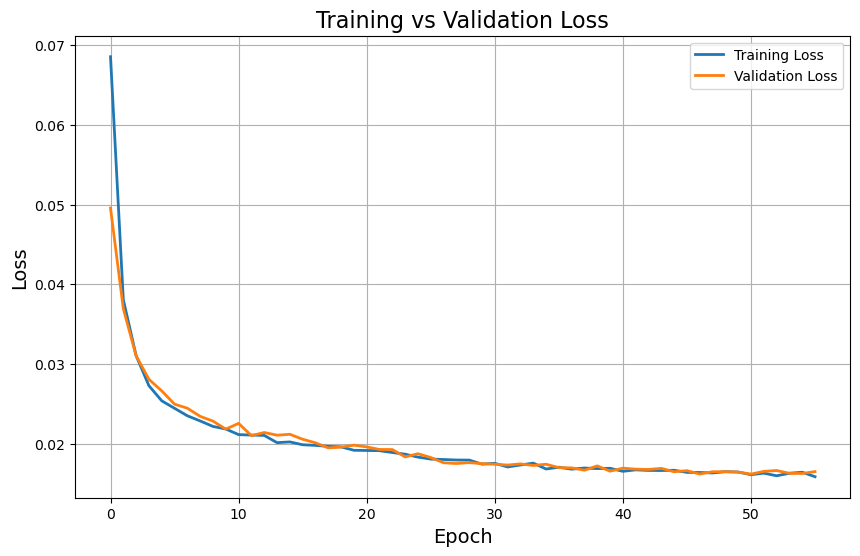
\includegraphics[width=1\linewidth]{figures/LSTM40_train_val_loss.png}
  \caption{Evolution of training and validation loss for LSTM40.}
  \label{fig:lossLSTM40}
\end{figure}

\subsubsection{Transformer} The training and validation performance of the base transformer and the big transformer models are shown in Figures \ref{fig:BaseT_train_val_loss} and \ref{fig:BigT_train_val_loss}. The first model trained for 106 epochs and resulted in a validation loss $4.4\times 10^{-6} $ at epoch number 86, while the second model trained for 161 models and resulted in a smaller validation loss of $3.8\times 10^{-6} $ at epoch 151.

\begin{figure}[htbp]
  \centering
  \includegraphics[width=1\linewidth]{figures/small_t_curve.png}
  \caption{Evolution of training and validation loss for Transformer-Base model.}
  \label{fig:BaseT_train_val_loss}
\end{figure}

\begin{figure}[htbp]
  \centering
  \includegraphics[width=1\linewidth]{figures/big_t_loss_curve.png}
  \caption{Evolution of training and validation loss for Transformer-Big model.}
  \label{fig:BigT_train_val_loss}
\end{figure}

\subsection{Test performance}

Lastly, we compare the performances of all models on a test set of plays the models have not observed, and for which we did not monitor the loss during the training stage. The experiment set up consists of using the last 100 pre-snap frames of each play in the test set to predict the trajectories of all players and the ball in the subsequent 40 frames. We believe that such window of prediction represents a trade-off between a sufficiently short time-frame in which can expect our models to produce reasonable trajectories, and a sufficiently long window so that the prediction would be informative for a team deciding on an offensive or defensive strategy.

For all the models except for LSTM40, predicting over a 40-frame window involves iteratively using the immediate next frame prediction as input for the subsequent prediction, until all the required predictions are obtained.

The error metric utilized for this experiment is \textit{Average Displacement Loss} (ADE), which is calculated in the same way as the MSE metric we used for training and validation, but we re-scaled the values to express them in yards, the original unit of the data, and averaged the loss per frame across the 22 players and the ball.

The model with the worst performance was LSTM1, with an average ADS of 4.35 yards. The next model was Base Transformer with an ADE of 1.74 yards. The Big Transformer model yielded an ADE of 1.30 yards. The best-performing model was LSTM40. with an ADE per player of 0.96 yards per frame.

We take this last result with caution as the experiment may be biased in favor of the model that was designed specifically to predict 40 frames ahead. To come to a more robust conclusion about which is the best performing model, we appeal to qualitative performance by visualizing the predicted trajectories of all models for the same play, and contrast it with the ground truth trajectories. This is important because the ADE metric does not necessarily reflect whether the predicted trajectories resemble the usual trajectories seen in real scenarios and playing strategies.

\section{Interpretation}

This section provides an interpretative analysis of the architectures implemented in our study, examining the predicted trajectories generated by different neural network models. All of the visualization in this section belong to the same play, with each model interpreting the pres-nap movement to predicting what it believes players will do once the ball is snapped.

\begin{figure}[htbp]
  \centering
  \includegraphics[width=1\linewidth]{figures/LSTM1_example_play.png}
  \caption{Model LSTM1: Predicted vs. actual player trajectories in an NFL play.}
  \label{fig:trajectoriesLSTM1}
\end{figure}

Figure \ref{fig:trajectoriesLSTM1} presents the trajectories generated by the LSTM1 model. The predicted trajectories from this simpler baseline architecture exhibit noticeable deviations, particularly in handling dynamic interactions among multiple players. The model yields a test loss of 1.817e-01, reflecting relatively limited predictive accuracy, particularly evident during complex player movements.

\begin{figure}[htbp]
  \centering
  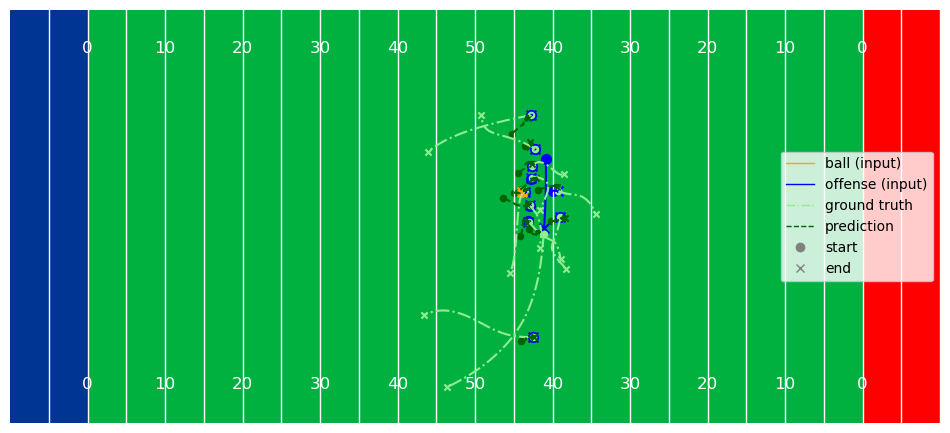
\includegraphics[width=1\linewidth]{figures/LSTM40_example_play.png}
  \caption{Model LSTM40: Predicted vs. actual player trajectories in an NFL play.}
  \label{fig:trajectoriesLSTM40}
\end{figure}

By contrast, Figure \ref{fig:trajectoriesLSTM40} illustrates the trajectories predicted by a more sophisticated variant, the LSTM40 model. Compared to LSTM1, the LSTM40 demonstrates significantly improved handling of trajectory prediction, better capturing the nuances of player movements and interactions. This improvement is quantitatively reflected in the considerably lower test loss of 1.622e-02.

\begin{figure}[htbp]
  \centering
  \includegraphics[width=1\linewidth]{figures/TransformerSmall_exmaple_play.jpeg}
  \caption{Transformer-Base: Predicted vs. actual player trajectories in an NFL play.}
  \label{fig:trajectoriesTSmall}
\end{figure}

Figure \ref{fig:trajectoriesTSmall} highlights the predictions from the Transformer-Base architecture. The Transformer demonstrates a marked ability to capture complex spatial-temporal dynamics, significantly outperforming the LSTM-based approaches. The model achieves a remarkably low test loss of 4.4058e-06, demonstrating its robust capacity for precise trajectory prediction, particularly in capturing long-range interactions and movements.

\begin{figure}[htbp]
  \centering
  \includegraphics[width=1\linewidth]{figures/TransformerBig_example_play.jpeg}
  \caption{Transformer-Big: Predicted vs. actual player trajectories in an NFL play.}
  \label{fig:trajectoriesTBig}
\end{figure}

Finally, Figure \ref{fig:trajectoriesTBig} shows the trajectories generated by the enhanced Transformer model (Transformer-Big). This more complex Transformer further refines the accuracy of trajectory predictions, yielding the lowest test loss of 3.8438e-06. The big Transformer effectively leverages deeper architectures to extract intricate patterns within the data, providing near-perfect alignment with observed trajectories.

The progressive reduction in test loss from LSTM-based models to Transformer-based architectures clearly highlights the effectiveness of incorporating attention mechanisms and deeper, more expressive structures. The transformer models' success underlines their suitability for modeling complex, dynamic interactions in sports scenarios, affirming their potential utility for practical, real-time analytics in American Football trajectory prediction.


\section{Conclusion}

In this paper, we explored the challenging task of trajectory prediction in American football using deep learning methods. Leveraging the NFL’s 2025 Big Data Bowl tracking dataset, we compared multiple architectures and implemented visualizations to demonstrate the predicted versus actual trajectories of given plays. Our results indicate that both Long Short-Term Memory networks and Transformer-based models are capable of producing accurate predictions of the trajectories for all 22 players and the ball following the snap, using only a brief pre-snap window of up to 10 seconds of movement. 

 Among the model architecture variants, our deep attention-based Transformer-Big model demonstrated the best performance with a MSE of $3.8\times 10^{-6} $, corresponding to an average positional deviation of approximately 1.3 yards per player.

These results underscore the potential of attention-based architectures in modeling multi-agent spatial-temporal interactions in structured sports like football. By conditioning only on pre-snap movement, our models align with real-world decision-making constraints, enabling predictive insights into opponent strategies and movements before the play begins.

While promising, our models are limited in the number of input features that they incorporate. In addition to the LSTM and transformer-based architectures listed above, we implemented a physics-informed Transformer variant that explicitly modeled motion dynamics through velocity and acceleration inputs. Rather than directly predicting future positional x and y coordinates, this physics-informed model output three meaningful quantities per agent: acceleration magnitude, direction sine, and direction cosine. These values, combined with each agent’s current position and velocity, are used to analytically compute the next position using basic kinematic equations.

We introduced a custom physics-informed loss function that penalizes the mean squared error between these computed next-frame positions and the actual ground-truth positions. This loss enforces a form of physical regularization, ensuring that predictions obey the laws of motion, improving interpretability and discouraging unrealistic outputs like sudden position jumps. However, by introducing over three times the number of input and model parameters, we quickly ran into computation and time constraints beyond the availability of this project. Greater computational resources such as utilizing distributive computing tools would be required to continue and compare the physics-informed transformer model. Future work could involve additional avenues of research such as incorporating contextual cues contained within the dataset that likely influence play design and player trajectory. These features include labels such as team formation (i.e., if a team known to prefer passing or running), player roles/physical characteristics (i.e., smaller faster wide receivers are more likely to run certain routes as compared to larger slower tight ends), or game state (i.e., plays near the goal-line are likely to involve vastly different player trajectories as compared to 3rd down and long near the end of a half). 

Ultimately, these tools could contribute to building intelligent systems that support real-time play diagnosis and game planning in competitive sports, pushing the evolution of strategy and data analytics forward.

\section{Bibliography}

\begin{thebibliography}{99}

\bibitem{Yu2020}
C. Yu, X. Ma, J. Ren, H. Zhao, and S. Yi, ``Spatio-Temporal Graph Transformer Networks for Pedestrian Trajectory Prediction,'' \textit{arXiv preprint arXiv:2005.08514}, 2020.

\bibitem{Mohamed2020}
A. Mohamed, K. Qian, M. Elhoseiny, and C. Claudel, ``Social-STGCNN: A Social Spatio-Temporal Graph Convolutional Neural Network for Human Trajectory Prediction,'' \textit{Proceedings of the IEEE/CVF Conference on Computer Vision and Pattern Recognition (CVPR)}, pp. 14424–14432, 2020.

\bibitem{Zhang2019}
P. Zhang, W. Ouyang, P. Zhang, J. Xue, and N. Zheng, ``SR-LSTM: State Refinement for LSTM Towards Pedestrian Trajectory Prediction,'' \textit{Proceedings of the IEEE/CVF Conference on Computer Vision and Pattern Recognition (CVPR)}, pp. 12077–12086, 2019.

\bibitem{Schmid2021}
M. Schmid, P. Blauberger, and M. Lames, ``Simulating Defensive Trajectories in American Football for Predicting League Average Defensive Movements,'' \textit{Frontiers in Sports and Active Living}, vol. 3, article 669845, 2021.

\bibitem{Fernandes2020}
C. J. Fernandes, R. Yakubov, Y. Li, A. K. Prasad, and T. C. Y. Chan, ``Predicting Plays in the National Football League,'' \textit{Journal of Sports Analytics}, vol. 6, no. 1, pp. 35–43, 2020.

\bibitem{Lopez2025}
Michael Lopez, Thompson Bliss, Ally Blake, Paul Mooney, and Addison Howard. NFL Big Data Bowl 2025. https://kaggle.com/competitions/nfl-big-data-bowl-2025, 2024. Kaggle.

\bibitem{Lurie2025}
"Jeffrey Lurie: Football is a chess match, let the chess match play out", NBC Sports, April 2025. https://www.nbcsports.com/nfl/profootballtalk/rumor-mill/news/jeffrey-lurie-football-is-a-chess-match-let-the-chess-match-play-out

\end{thebibliography}

\section{Statement about individual contributions}

Candidate 37269: 
Literature review, data exploration, visualizations, model training, model evaluation, writing.
\\
Candidate 38682:
Introduction, literature review, physics-based loss model training, writing.
\\
Candidate 46679:
Project idea, data pipeline, Transformer model creation and training, writing. 
\\
Candidate 40658:
Literature review, LSTM model creation and training, writing.
\\
Each member contributed equally to the project.
\\
\section{Statement about the use of generative AI and chat logs}

The chatbot tool ChatGPT, in its various versions, has been used extensively to aid the coding section and the writing of the project.

\end{document}
\endinput
%%
%% End of file `sample-sigconf.tex'.







} (shared \(300\)-unit cell)